\section{Neural Networks}
\begin{itemize}
	\item Previously: fixed basis function $\bm{\phi}(\bm{x}) = \left(\phi_0\left(\bm{x}\right), \phi_1\left(\bm{x}\right), ..., \phi_M\left(\bm{x}\right)\right)^T$
	\item Neural networks: Create flexible non-linear features and learn them. 
	\begin{itemize}
		\item Basis function with extra parameters: $\phi_m\left(\bm{x},\bm{w}_m^{(1)}\right) = h\left(\left(\bm{w}_m^{(1)}\right)^T \bm{x}\right) = h\left(\sum\limits_{d=0}^{D}w_{md}^{(1)}\right)$ 
		\item Note that $\bm{x}_n = \left(1, x_{n0},...,x_{nD}\right)^T\Rightarrow \bm{x}_n \in \mathbb{R}^D$
		\item $h$ is the non-linear activation function
	\end{itemize}
	\item We can define regression for a one-layer neural network:
	\begin{equation*}
		\begin{split}
			y\left(\bm{x}, \bm{W}^{(1)}, \bm{w}^{(2)}\right) & = \sum\limits_{m=0}^{M} w_m^{(2)} h\left(\sum\limits_{d=0}^{D}w_{md}^{(1)}\right) \\
			& = \left(\bm{w}^{(2)}\right)^T h\left(\bm{W}^{(1)} \bm{x}\right) \text{\hspace{5mm}where\hspace{5mm}} \bm{W}^{(1)} = \left(\begin{array}{cccc}
			\mid & \mid & \dots & \mid\\
			\bm{w}_0^{(1)} & \bm{w}_1^{(1)} & \dots & \bm{w}_D^{(1)}\\
			\mid & \mid & \dots & \mid
			\end{array}\right)\\
		\end{split}
	\end{equation*}
	\item The same way, we can adjust a network for classification:
	$$y\left(\bm{x}, \bm{W}^{(1)}, \bm{w}^{(2)}\right) = f\left(\sum\limits_{m=0}^{M} w_m^{(2)} h\left(\sum\limits_{d=0}^{D}w_{md}^{(1)}\right)\right) = f\left(\left(\bm{w}^{(2)}\right)^T h\left(\bm{W}^{(1)} \bm{x}\right)\right)$$
	where $f$ is sigmoid for binary and softmax for multi-class classification (then $\bm{w}^{(2)}$ is $K\times M$ matrix)
\end{itemize}
\subsection{Feed-forward Network Functions}
\begin{itemize}
	\begin{figure}[ht]
		\centering
		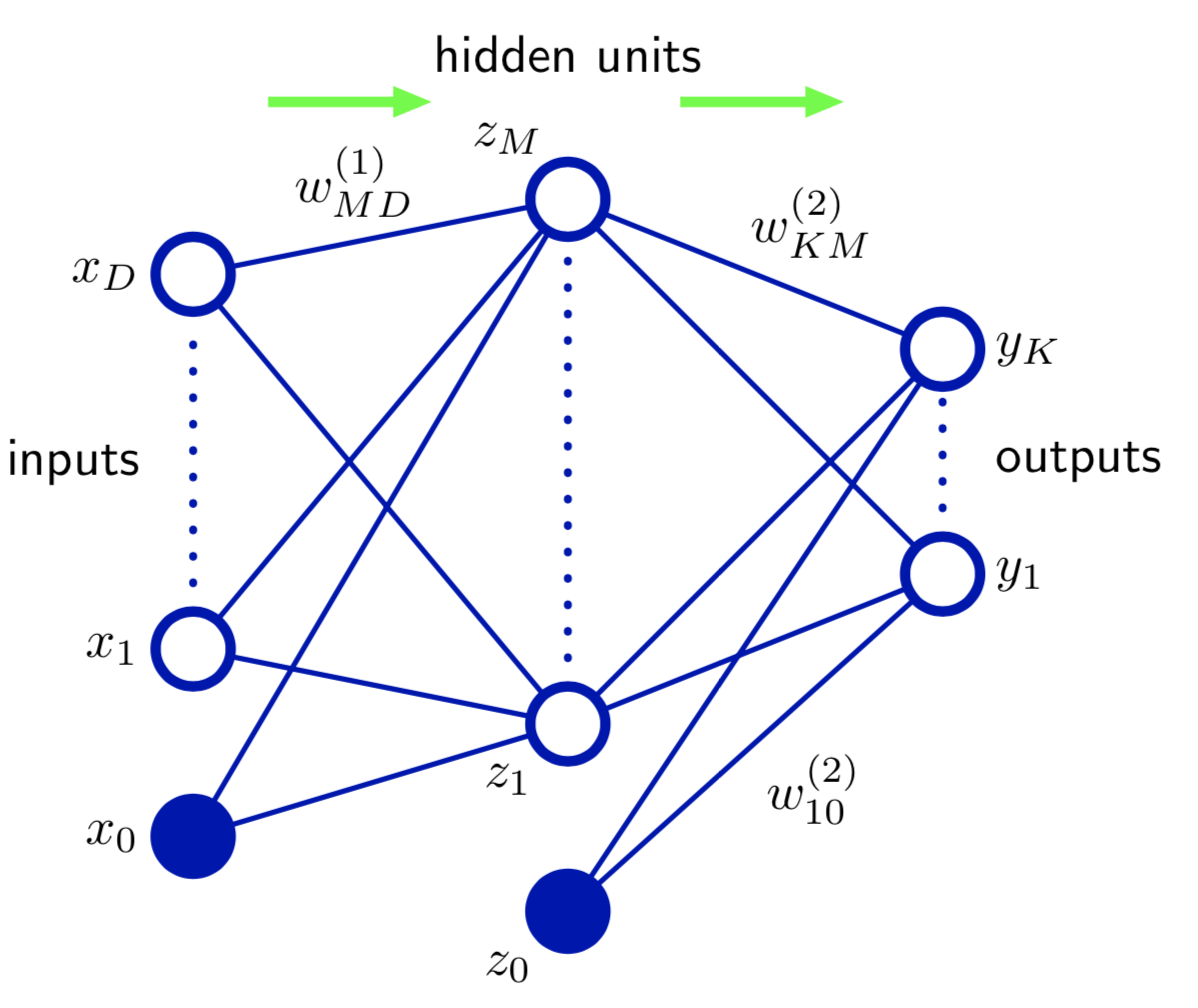
\includegraphics[width=0.5\textwidth]{figures/neural_networks_overview.png}
		\caption{Illustration of a multilayer perceptron (2 layers).}
		\label{img:neural_networks_overview}
	\end{figure}
	\item Input are $D+1$ units whereas $x_0=1$ is the bias
	\item First layer with $M\times D$ weight matrix $\bm{W}^{(1)}$ $\Rightarrow$ $M$ activations $a_m = \sum\limits_{d=0}^{D} w_{md}^{(1)} x_{d}$ and bias $h^{(1)}(a_0)=1$
	\item We apply an activation function on these activations to get the hidden units: $z_m = h^{(1)}(a_m)$ where $z_0=1$
	\item Second layer with $K\times M$ weight matrix $\bm{W}^{(2)}$ $\Rightarrow$ $K$ output units $y_k = h^{(2)}\left(\sum\limits_{m=0}^{M} w_{km}^{(2)}z_m\right)$
	\item In conclusion, a output unit $y_k$ is calculated as follows:
	$$y_k\left(\bm{x}, \bm{W}^{(1)}, \bm{W}^{(2)}\right) = h^{(2)}\left(\sum\limits_{m=0}^{M} w_{km}^{(2)}\cdot h^{(1)}\left(\sum\limits_{d=0}^{D} w_{md}^{(1)}x_{d}\right)\right)$$
	\item Alternative notation: $y_k = h^{(2)} \circ \bm{a}^{(2)} \circ h^{(1)} \circ \bm{a}^{(1)} (\bm{x})$
	\item Additional forms: 
	\begin{itemize}
		\item \textit{Skip connections}: Connection between for instance first and fourth layer
		\item \textit{Sparse connections}: For instance convolutions, can have weight sharing
	\end{itemize}
	\item In general: $z_m = h\left(\sum\limits_{j}w_{mj}z_{j}\right)$ where $j$ are all incoming connections
	\item Note that no closed directed cycles are allowed
\end{itemize}
\subsubsection{Universal approximator}
\begin{itemize}
	\item Let $f$ by any continuous function on a compact area of $\mathbb{R}^{D}$ and $h$ any fixed analytic function which is not polynomial (e.g. logistic function, tanh function, ...). Given any small number $\epsilon > 0$ of an acceptable error, we can find a number $M$ and weights $w_{m}^{(2)}$ and $w_{md}^{(1)}\in \mathbb{R}$ such that:
	$$\left|f(\bm{x}) - y\left(\bm{x}, \bm{W}^{(1)}, \bm{w}^{(2)}\right)\right| < \epsilon$$
	with $y$ as two-layer NN
	\item For smaller $\epsilon$ we need more hidden units $\Rightarrow$ larger $M$
	\item We may also take deeper networks that are usually capable to approximate more complex functions with less units
	\item To approximate deep network with shallow one by error $\epsilon$, the number of units $M$ needed scales exponentially for decreasing $\epsilon$
	\begin{figure}[ht]
		\centering
		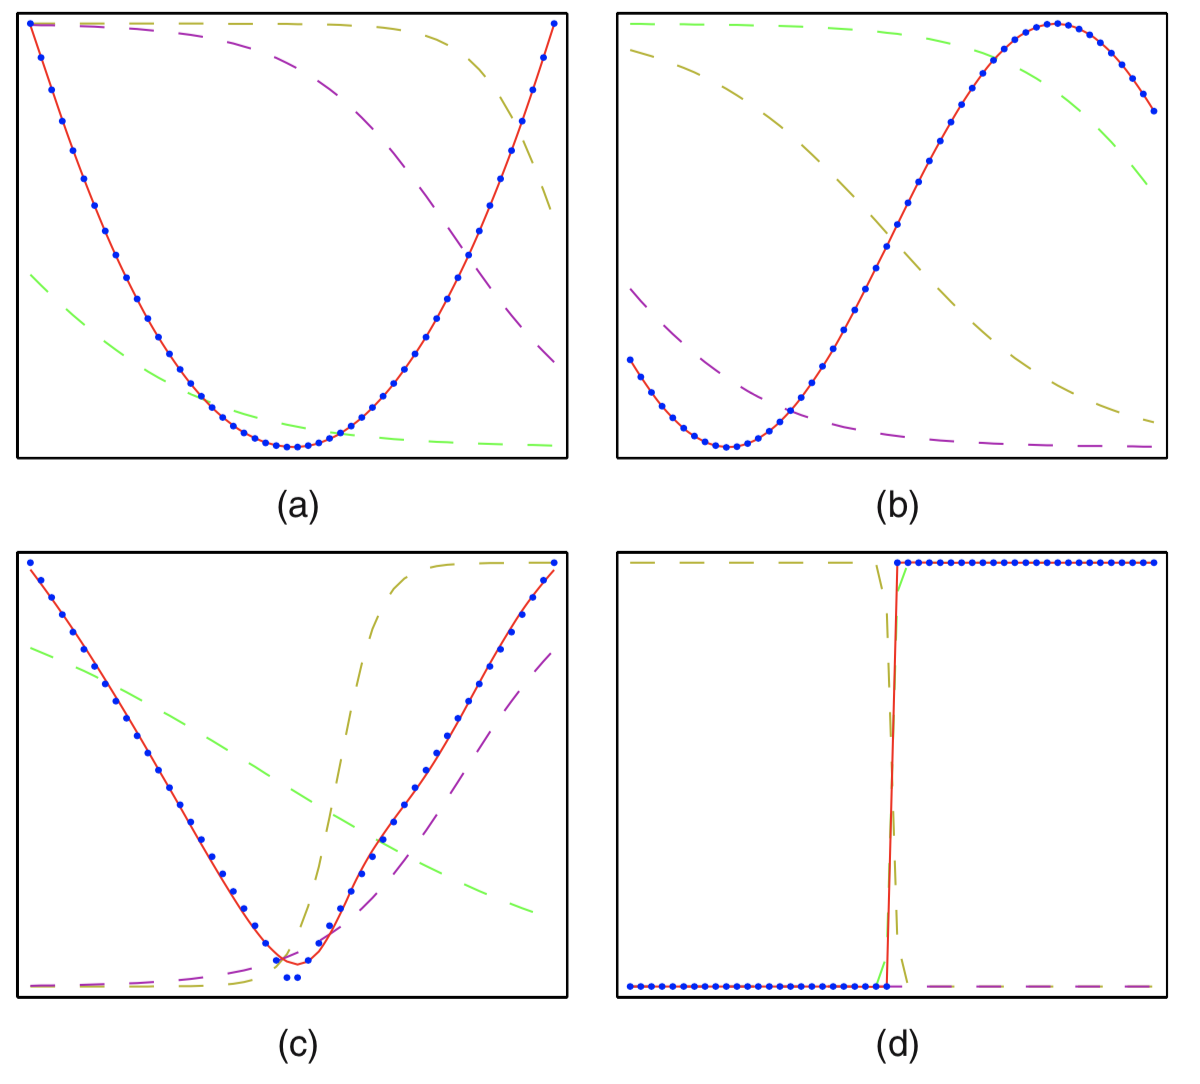
\includegraphics[width=0.4\textwidth]{figures/neural_networks_universal_approximator.png}
		\caption{Example approximations by a 2-layer network with 3 hidden units of the function (a) $f(x)=x^2$, (b) $f(x)=\sin(x)$, (c) $f(x) = |x|$ and (d) $f(x)=\mathbb{I}\left(x>0\right)$. The outputs of the three hidden units are shown as dashed lines.}
		\label{img:neural_networks_universal_approximator}
	\end{figure}
\end{itemize}
\subsection{Network Training}
\begin{itemize}
	\item Use probabilistic interpretation of the network outputs to choose number of outputs, output activation function and loss (e.g. $p(t|\bm{x},\bm{w})$ for regression $\Rightarrow$ maximizing likelihood used as error function)
\end{itemize}
\subsubsection{Network training for regression}
\begin{itemize}
	\item Data input $\bm{x}_n \in \mathbb{R}^{D}$ with continuous target $t_n \in \mathbb{R}$
	\item Single real-valued target $\to$ Single output unit with identity activation function $y\left(\bm{x}, \bm{w}\right) = a^{\text{out}}$
	\item Derive loss function by maximum likelihood:
	$$E(\bm{w}) = -\ln p\left(\bm{t}|\bm{X}, \bm{w}\right) = \frac{\beta}{2}\sum\limits_{n=1}^{N}\left\{y(\bm{x}_n, \bm{w}) - t_n\right\}^2 - \frac{N}{2}\ln\beta + \frac{N}{2}\ln 2\pi $$
	$$\text{equivalent to minimizing } E(\bm{w})=\frac{1}{2}\sum\limits_{n=1}^{N}\left\{y(\bm{x}_n, \bm{w}) - t_n\right\}^2$$
\end{itemize}
\subsubsection{Network training for binary classification}
\begin{itemize}
	\item Targets are now binary values: $t_n\in\left\{0,1\right\}$
	\item As $p\left(t=1|\bm{x}\right) = 1 - p\left(t=0|\bm{x}\right)$, we model only one output unit: $y\left(\bm{x},\bm{w}\right) = p\left(t=1|\bm{x}\right)$
	\item The output activation function is therefore a sigmoid: $y\left(\bm{x}, \bm{w}\right) = \sigma\left(a^{\text{out}}\right)$
	\item The maximum likelihood is here equivalent to minimizing BCE: $$E\left(\bm{w}\right) = -\sum\limits_{n=1}^{N} t_n \ln y\left(\bm{x}_n, \bm{w}\right) + (1 - t_n) \ln \left(1 - y\left(\bm{x}_n, \bm{w}\right)\right)$$
\end{itemize}
\subsubsection{Network training for classification with $K$ classes}
\begin{itemize}
	\item Targets are now one-hot vectors $\bm{t}_n = \left(0,...,1,...,0\right)^T$
	\item Now, we have to model all $K$ class distributions by $y_k\left(\bm{x}, \bm{w}\right) = p\left(C_k|\bm{x}\right)$
	\item Activation function is softmax: $y_k\left(\bm{x}, \bm{w}\right) = \frac{\exp\left(a_k^{\text{out}}\right)}{\sum_{j=1}^{K}\exp\left(a_j^{\text{out}}\right)}$
	\item The maximum likelihood is here equivalent to:
	$$E\left(\bm{w}\right) = - \sum\limits_{n=1}^{N} \sum\limits_{k=1}^{K} t_{nk} \ln y_k\left(\bm{x}_n, \bm{w}\right)$$
\end{itemize}
\subsubsection{Parameter optimization}
\begin{itemize}
	\item Optimal parameters minimize error function: $\bm{w}^{*} = \arg\min\limits_{\bm{w}} E(\bm{w})$
	\item Problem: $E(\bm{w})$ is not convex so that many local minima (can) exist 
	\item Different optimization strategies can be developed
	\item \textbf{Gradient Descent} uses full dataset for each update: $\bm{w}^{(\tau + 1)} = \bm{w}^{(\tau)} - \eta \triangledown E\left(\bm{w}^{(\tau)}\right)$
	\item Always goes in the direction of steepest gradient
	\item Will easily get stuck in local minimum when $\triangledown E\left(\bm{w}\right) = 0$
	\item \textbf{Stochastic Gradient Descent} uses single data point or minibatches for the update step: $\bm{w}^{(\tau + 1)} = \bm{w}^{(\tau)} - \eta \triangledown\sum\limits_{i=1}^{M} E_i\left(\bm{w}^{(\tau)}\right)$ 
	\item Converges to area around local minimum
	\item More likely to escape local minimum as $\triangledown E\left(\bm{w}^{(\tau)}\right) = 0$ does not imply $\triangledown E_n\left(\bm{w}^{(\tau)}\right) = 0$ for all $n$
	\item Is more computational efficient at the beginning as all $E_n\left(\bm{w}\right)$ will point in a similar direction
	\item Choose learning rate carefully to get good results
	\begin{itemize}
		\item If learning rate is too small: slow convergence
		\item If learning rate is too high: oscillations around local minimum
		\item Use learning rate scheduling with smaller learning rate over time
	\end{itemize}
\end{itemize}
\subsection{Error Backpropagation}
\begin{itemize}
	\item The error function is the sum of single point errors ($E(\bm{w})=\sum_{n}E_n(\bm{w})$), so that we can calculate the gradients for each data point independently: $\frac{\partial E_n(\bm{w})}{\partial \bm{w}}$ 
	\item Therefore, we first apply \textit{forward propagation}: calculate all $a_j^{(l)} = \sum_i w_{ji}^{(l)}z_i^{(l-1)}$ and $z_j^{(l)}=h^{(l)}\left(a_j^{(l)}\right)$
	\item Then, apply \textit{back propagation} by calculating all $\frac{\partial E_n}{\partial w_{ji}^{(l)}}$
	\item Backpropagation is based on the multi-dimensional chain rule: 
	$$\frac{\partial f\left(g_1\left(x\right), ..., g_D\left(x\right) \right)}{\partial x} = \sum\limits_{d=1}^{D}\frac{\partial f\left(g_1\left(x\right), ..., g_D\left(x\right)\right)}{\partial g_d(x)}\frac{\partial g_d(x)}{\partial x}$$
	\item Thus, we can express the gradient regarding a single weight element by (only $a_{j}^{(l)}$ depends on $w_{ji}^{(l)}$):
	$$\frac{\partial E_n}{\partial w_{ji}^{(l)}}=\frac{\partial E_n}{\partial a_{j}^{(l)}}\frac{\partial a_{j}^{(l)}}{\partial w_{ji}^{(l)}}$$
	\item The second part of the derivate is just $\frac{\partial a_{j}^{(l)}}{\partial w_{ji}^{(l)}}=z_{i}^{(l-1)}$, the first one we define as $\delta_j^{(l)}\equiv \frac{\partial E_n}{\partial a_j^{(l)}}$
	\item So, our derivate is $\frac{\partial E_n}{\partial w_{ji}^{(l)}}=\delta_j^{(l)}z_{i}^{(l-1)}$
	\item $a_j^{(l)}$ effects the error only by its following units $a_k^{(l+1)}\Rightarrow \delta_j^{(l)}=\sum_{k}\frac{\partial E_n}{\partial a_k^{(l+1)}}\frac{\partial a_k^{(l+1)}}{a_j^{(l)}} = \sum_{k}\delta_{k}^{(l+1)}\frac{\partial a_k^{(l+1)}}{a_j^{(l)}}$
	\item As $a_j^{(l)}$ effects $a_k^{(l+1)}$ only by the weight $w_{kj}^{(l+1)}$, the derivate is $\frac{\partial a_k^{(l+1)}}{a_j^{(l)}}=w_{kj}^{(l+1)}h^{(l)'} \left(a_{j}^{(l)}\right)$
	\item Note that we need to be careful with skip connections
	\item Overall, backpropagation can be summarized in three steps:
	\begin{enumerate}
		\item Compute $\delta_k$ for all output units
		\item Compute $\delta_j$ for all hidden units through backpropagation:
		$$\delta_j^{(l)} = h^{(l)'}\left(a_j^{(l)}\right)\sum\limits_{k}\delta_k^{(l+1)}w_{kj}^{(l+1)}$$
		\item Compute derivatives $\frac{\partial E_n}{\partial w_{ji}^{(l)}}=\delta_j^{(l)}z_{i}^{(l-1)}$
		\item Apply iterative weight update: 
		$w_{ji}^{(l)(\tau+1)} = w_{ji}^{(l)(\tau)}-\eta \delta_j^{(l)}z_{i}^{(l-1)}$
	\end{enumerate}
\end{itemize}
\subsection{Issues with Neural Networks}
\begin{itemize}
	\item Initialization of weights: randomly start near zero such that activations fall into linear part of activation functions (e.g. for tanh and sigmoid) and gradients don't vanish
	\item Networks perform best when input has mean 0 and variance 1
	\item When you have a large number of parameters, we need regularization!
	\item Multiple local minima: Non-convex error function. Restart experiment with different seeds and choose model with lowest regularized error
	\item Use weight sharing to reflect symmetries in data if possible
\end{itemize}